\documentclass[12pt, a4paper]{article}

% Packages dependencies
\usepackage[brazil]{babel}
\usepackage[top=3cm, bottom=2cm, left=3cm, right=3cm]{geometry}
\usepackage{graphicx}
\usepackage{titlesec}
\usepackage{float}
\usepackage{minted}
\usepackage{xcolor}
\usepackage[labelformat=empty]{caption}
\usepackage{amsmath}
\usepackage{amssymb}
\usepackage{fontspec}
\usepackage{multicol}
\usepackage{indentfirst}
\usepackage{hyperref}
\usepackage{titlesec}
\usepackage{enumitem}
\usepackage[most]{tcolorbox}
\usepackage{cleveref}
\hypersetup{
    colorlinks=true,
    urlcolor=blue,
    linkcolor=blue
}
\setmainfont{ARIAL.TTF}[
  ItalicFont = ARIALI.TTF,
  BoldFont = ARIALBD.TTF,
  BoldItalicFont = ARIALBI.TTF,
  Path = ./fontes/
]
\setmonofont{JetBrains Mono}[
Scale=MatchLowercase,
Ligatures=TeX,
Contextuals=Alternate
]
\newtcolorbox{mybox}[2][]{breakable,sharp corners, skin=enhancedmiddle jigsaw,parbox=false,
boxrule=0mm,leftrule=2mm,boxsep=0mm,arc=0mm,outer arc=0mm,attach title to upper,
after title={.\ }, coltitle=black,colback=gray!10,colframe=black, title={#2},
fonttitle=\bfseries,#1}
\renewcommand*\contentsname{SUMÁRIO}

\graphicspath{{images/}}

%Preamble
\date{\today}

%Variable Student Name
\newcommand\studentName{Matheus de Freitas Weber}
\newcommand\studentTwoName{Gabriel Berwanger Silveira}
\newcommand\studentThreeName{Aluno 3}
\newcommand\studentFourName{Aluno 4}

%Variable Course Name
\newcommand\courseName{Circuitos microprocessados}

%Variable Article Name
\newcommand\titleName{Exercício - Aula 03}

%Variable Article SubName
\newcommand\subTitleName{Sistema Cliente-Servidor e comunicação serial}

%Variable Teacher Name
\newcommand\teacherName{Jean Schmith}

%Body
\begin{document}

% -- Unisinos title -- %
\begin{center}
	\MakeUppercase{\textbf{Universidade do Vale do Rio dos Sinos (Unisinos)}}

	% -- Course Name -- %
	\MakeUppercase{\textbf{Graduação em Engenharia de controle e automação}} \\[16ex]


	% -- Student Name -- %
	\MakeUppercase{\textbf{\studentName}}
	\\
	\MakeUppercase{\textbf{\studentTwoName}}
	\\[16ex]

	% -- Work Title -- %
	\MakeUppercase{\textbf{\titleName}}

	\textbf{\subTitleName}

	\vfill

	\textbf{São Leopoldo}

	\textbf{2025}

	\thispagestyle{empty}
\end{center}
\newpage

% -- Capa -- %
\begin{center}
	% -- Capa -- %
	\vspace*{28ex}
	\MakeUppercase{\studentName}
	\\
	\MakeUppercase{\studentTwoName}
	\vspace*{16ex}

	\MakeUppercase{\textbf{\titleName}}

	\textbf{\subTitleName}

	\vspace*{8ex}

	% -- Description of the work -- %
	\hfill\begin{minipage}{0.5\linewidth}
		Trabalho apresentado para a matéria {\courseName} pelo Curso de Engenharia de Controle e Automação e Engenharia da Computação da Universidade do Vale do Sinos (UNISINOS), ministrada pelo Prof.\teacherName.
	\end{minipage}
	\vfill

	\textbf{São Leopoldo}

	\textbf{2025}

\end{center}
\thispagestyle{empty}
\setcounter{page}{1}

\newpage
% -- Summary -- %
\begin{center}
	\tableofcontents
\end{center}
\thispagestyle{empty}

\newpage
% -- Introduction -- %
\section{Introdução}
Em sistemas embarcados a compreensão da comunicação entre microcontroladores e integração efeciente entre hardware e software é essencial. Entro os modelos utilizados nesse contexto destaca-se a arquitetura Cliente-Servidor que permite centralizar o controle, dessa forma coordenando o funcionamento das unidades subordinadas.

Neste trabalho, exploramos a implementação de um sistema de comunicação serial entre três microcontroladores associando o uso de GPIOs como chip select para a correta identificação dos dispositivos que devem responder aos comandos enviados. Através de botões físicos vinculados aos microcontroladores do tipo cliente o usuário pode fazer o acionamento e desligamento individual dos LEDs conectados ao microcontrolador correspondente. O microcontrolador do tipo servidor é responsável por receber os comandos e repassá-los aos clientes corretos, garantindo a execução das ações solicitadas.

\newpage
% -- Teorical foundation -- %
\section{Fundamentação teórica}
\subsection{Arquitetura Cliente-Servidor}
A arquitetura Cliente-Servidor é um modelo de comunicação onde um dispositivo (o cliente) solicita serviços ou recursos de outro dispositivo (o servidor). O servidor é responsável por fornecer esses serviços ou recursos, enquanto o cliente inicia a comunicação e faz as solicitações. Essa arquitetura é amplamente utilizada em redes de computadores, sistemas distribuídos e aplicações web.
\subsection{Comunicação Serial}
A comunicação serial é um método de transmissão de dados onde os bits são enviados sequencialmente, um após o outro, através de um único canal de comunicação. Esse método é eficiente para longas distâncias. Para comunicação entre microcontroladores é necessário definir parâmetros como taxa de transmissão (baud rate), paridade, bits de dados e bits de parada para garantir a integridade dos dados transmitidos.
\subsection{GPIO (General Purpose Input/Output)}
GPIOs são pinos de um microcontrolador que podem ser configurados como entradas ou saídas digitais. Eles são usados para interagir com outros dispositivos eletrônicos, como sensores, atuadores e outros microcontroladores. Em sistemas embarcados, os GPIOs são essenciais para a comunicação e controle de hardware.
\subsection{Chip Select (CS)}
O Chip Select (CS) é um sinal utilizado em sistemas de comunicação serial para selecionar um dispositivo específico em um barramento compartilhado. Quando o CS está ativo (geralmente em nível baixo), o dispositivo selecionado está habilitado para comunicação, enquanto os outros dispositivos permanecem inativos. Isso é crucial em sistemas onde múltiplos dispositivos compartilham a mesma linha de dados.
\subsection{Microcontroladores}
Microcontroladores são pequenos computadores em um único chip que contêm um processador, memória e periféricos de entrada/saída. Eles são amplamente utilizados em sistemas embarcados para controlar dispositivos eletrônicos, executar tarefas específicas e interagir com o ambiente.

\newpage
\section{Metodologia}
\subsection{Materiais Utilizados}
\begin{itemize}
	\item 2x Placas Arduino Uno R3
	\item 2x LEDs
	\item 2x Resistores 330Ω
	\item 2x Botões (Push Buttons)
	\item Fios de conexão (Jumpers)
	\item Protoboard (opcional)
\end{itemize}

\subsection{Diagrama de Conexões}
\begin{figure}[H]
	\centering
	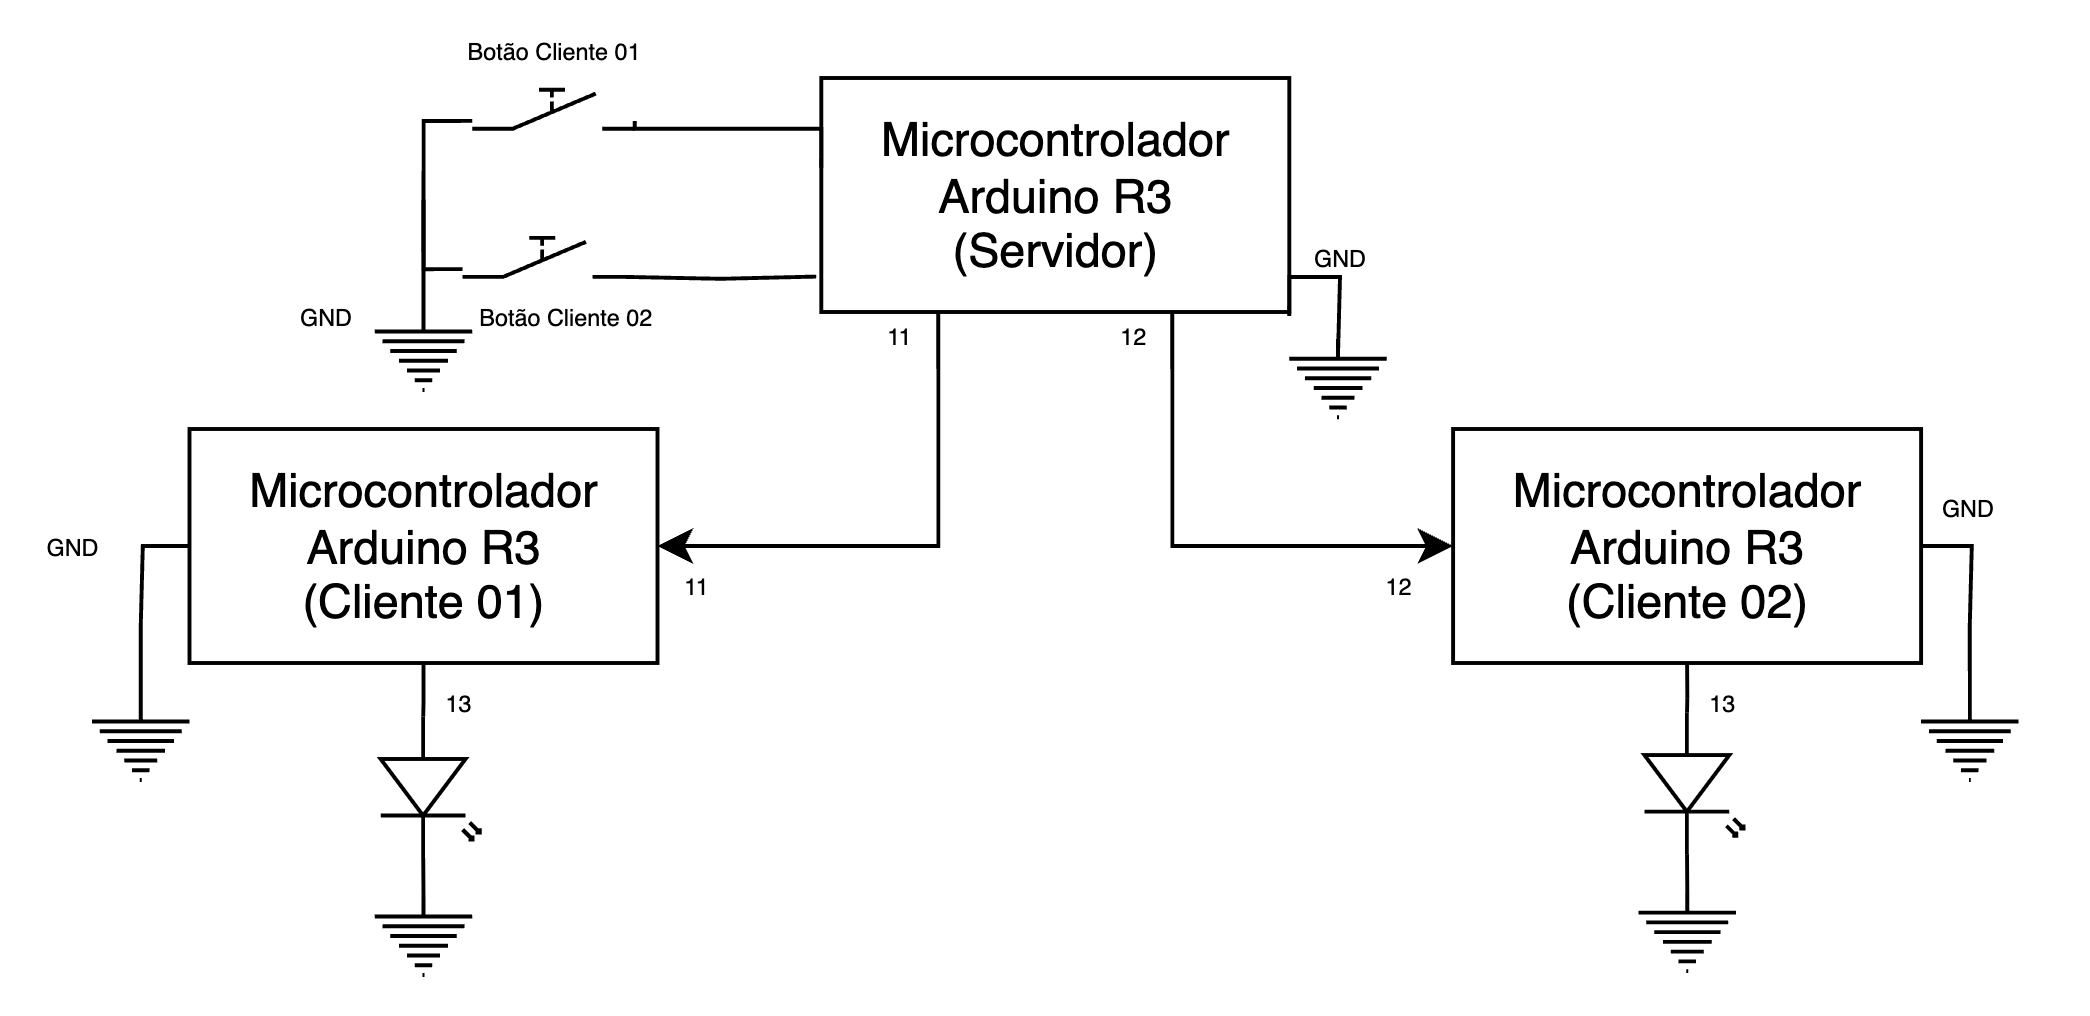
\includegraphics[width=0.8\textwidth]{diagrama_conexoes.png}
	\caption{Diagrama de conexões entre os microcontroladores, LEDs e botões.}
	\label{fig:diagrama_conexoes}
\end{figure}
\subsection{Configuração dos Microcontroladores}
\subsubsection{Microcontrolador Servidor}
O microcontrolador servidor é responsável por receber os comandos dos microcontroladores clientes e repassá-los para os dispositivos corretos. Ele utiliza a comunicação serial para interagir com os clientes e controla os GPIOs para selecionar o dispositivo correto através do sinal Chip Select (CS).
\begin{figure}[H]
	\centering
	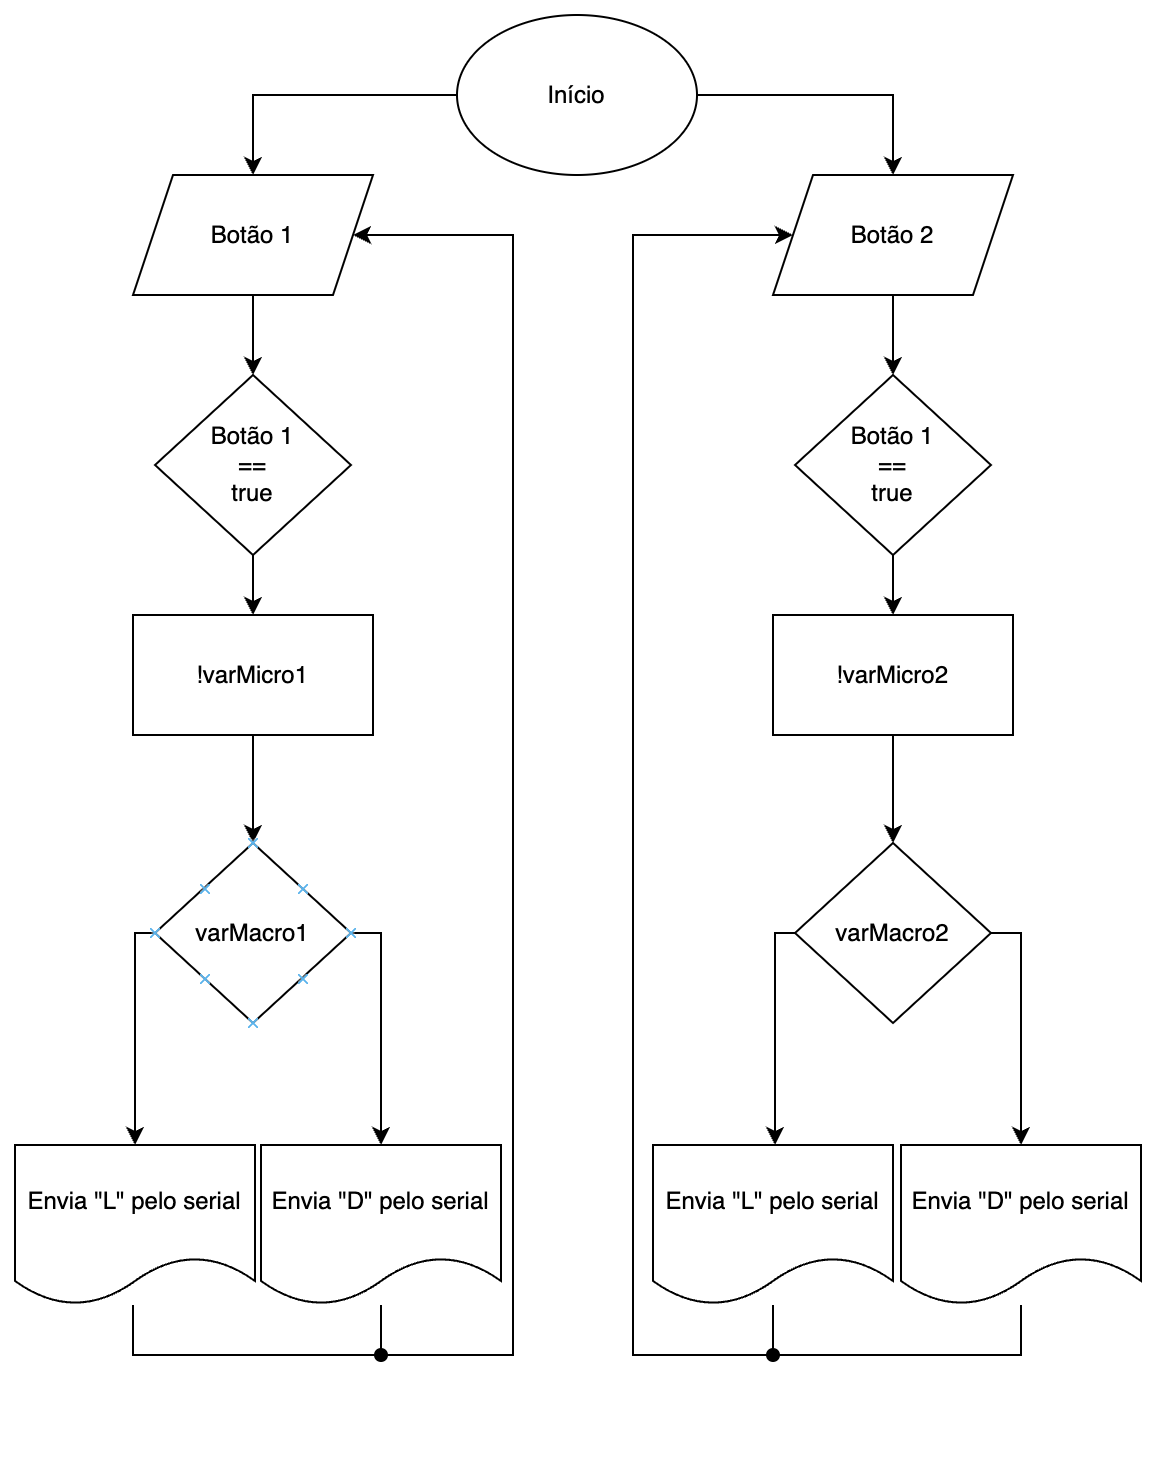
\includegraphics[width=0.8\textwidth]{fluxograma_servidor.png}
	\caption{Fluxograma do microcontrolador servidor.}
	\label{fig:fluxograma_servidor}
\end{figure}
\subsubsection{Microcontroladores Clientes}
Os microcontroladores clientes são responsáveis por monitorar os botões físicos e enviar comandos ao microcontrolador servidor quando um botão é pressionado. Cada cliente está associado a um LED específico, que será acionado ou desligado com base nos comandos recebidos do servidor.
\begin{figure}[H]
	\centering
	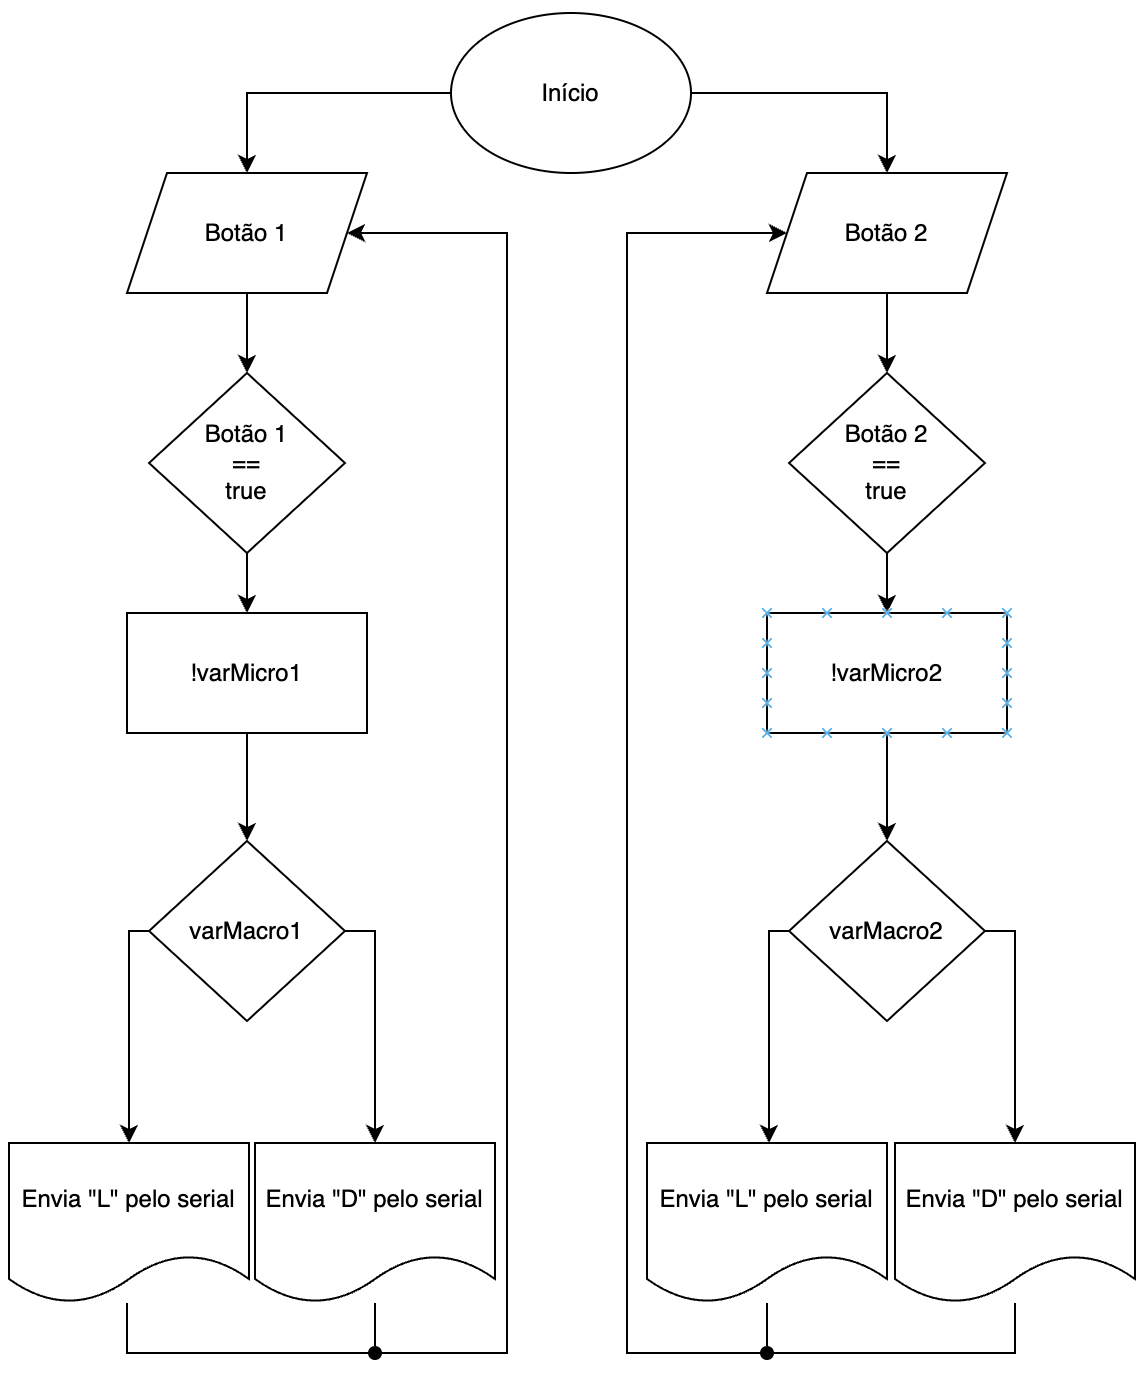
\includegraphics[width=0.8\textwidth]{fluxograma_cliente.png}
	\caption{Fluxograma do microcontrolador cliente.}
\end{figure}
\label{fig:fluxograma_cliente}
\subsection{Implementação do Código}
\subsubsection{Código do Microcontrolador Servidor}
\begin{mybox}[label={lst:codigo_servidor},title={Código do Microcontrolador Servidor}]{}
	\inputminted[fontsize=\footnotesize,breaklines,linenos]{cpp}{./arduino/codigo_servidor/codigo_servidor.ino}
\end{mybox}
\subsubsection{Código do Microcontrolador Cliente}
\begin{mybox}[label={lst:codigo_cliente},title={Código do Microcontrolador Cliente}]{}
	\inputminted[fontsize=\footnotesize,breaklines,linenos]{cpp}{./arduino/codigo_cliente/codigo_cliente.ino}
\end{mybox}
\newpage
\section{Resultados}
Através da implementação do sistema de comunicação serial entre os microcontroladores, foi possível observar o funcionamento correto da arquitetura Cliente-Servidor. Os microcontroladore servidor foram capazes de enviar comandos aos clientes quando os botões foram pressionados preservando seus estados tornando o efeito 'toggle', e o servidor respondeu adequadamente acionando ou desligando os LEDs correspondentes.
\begin{figure}[H]
	\centering
	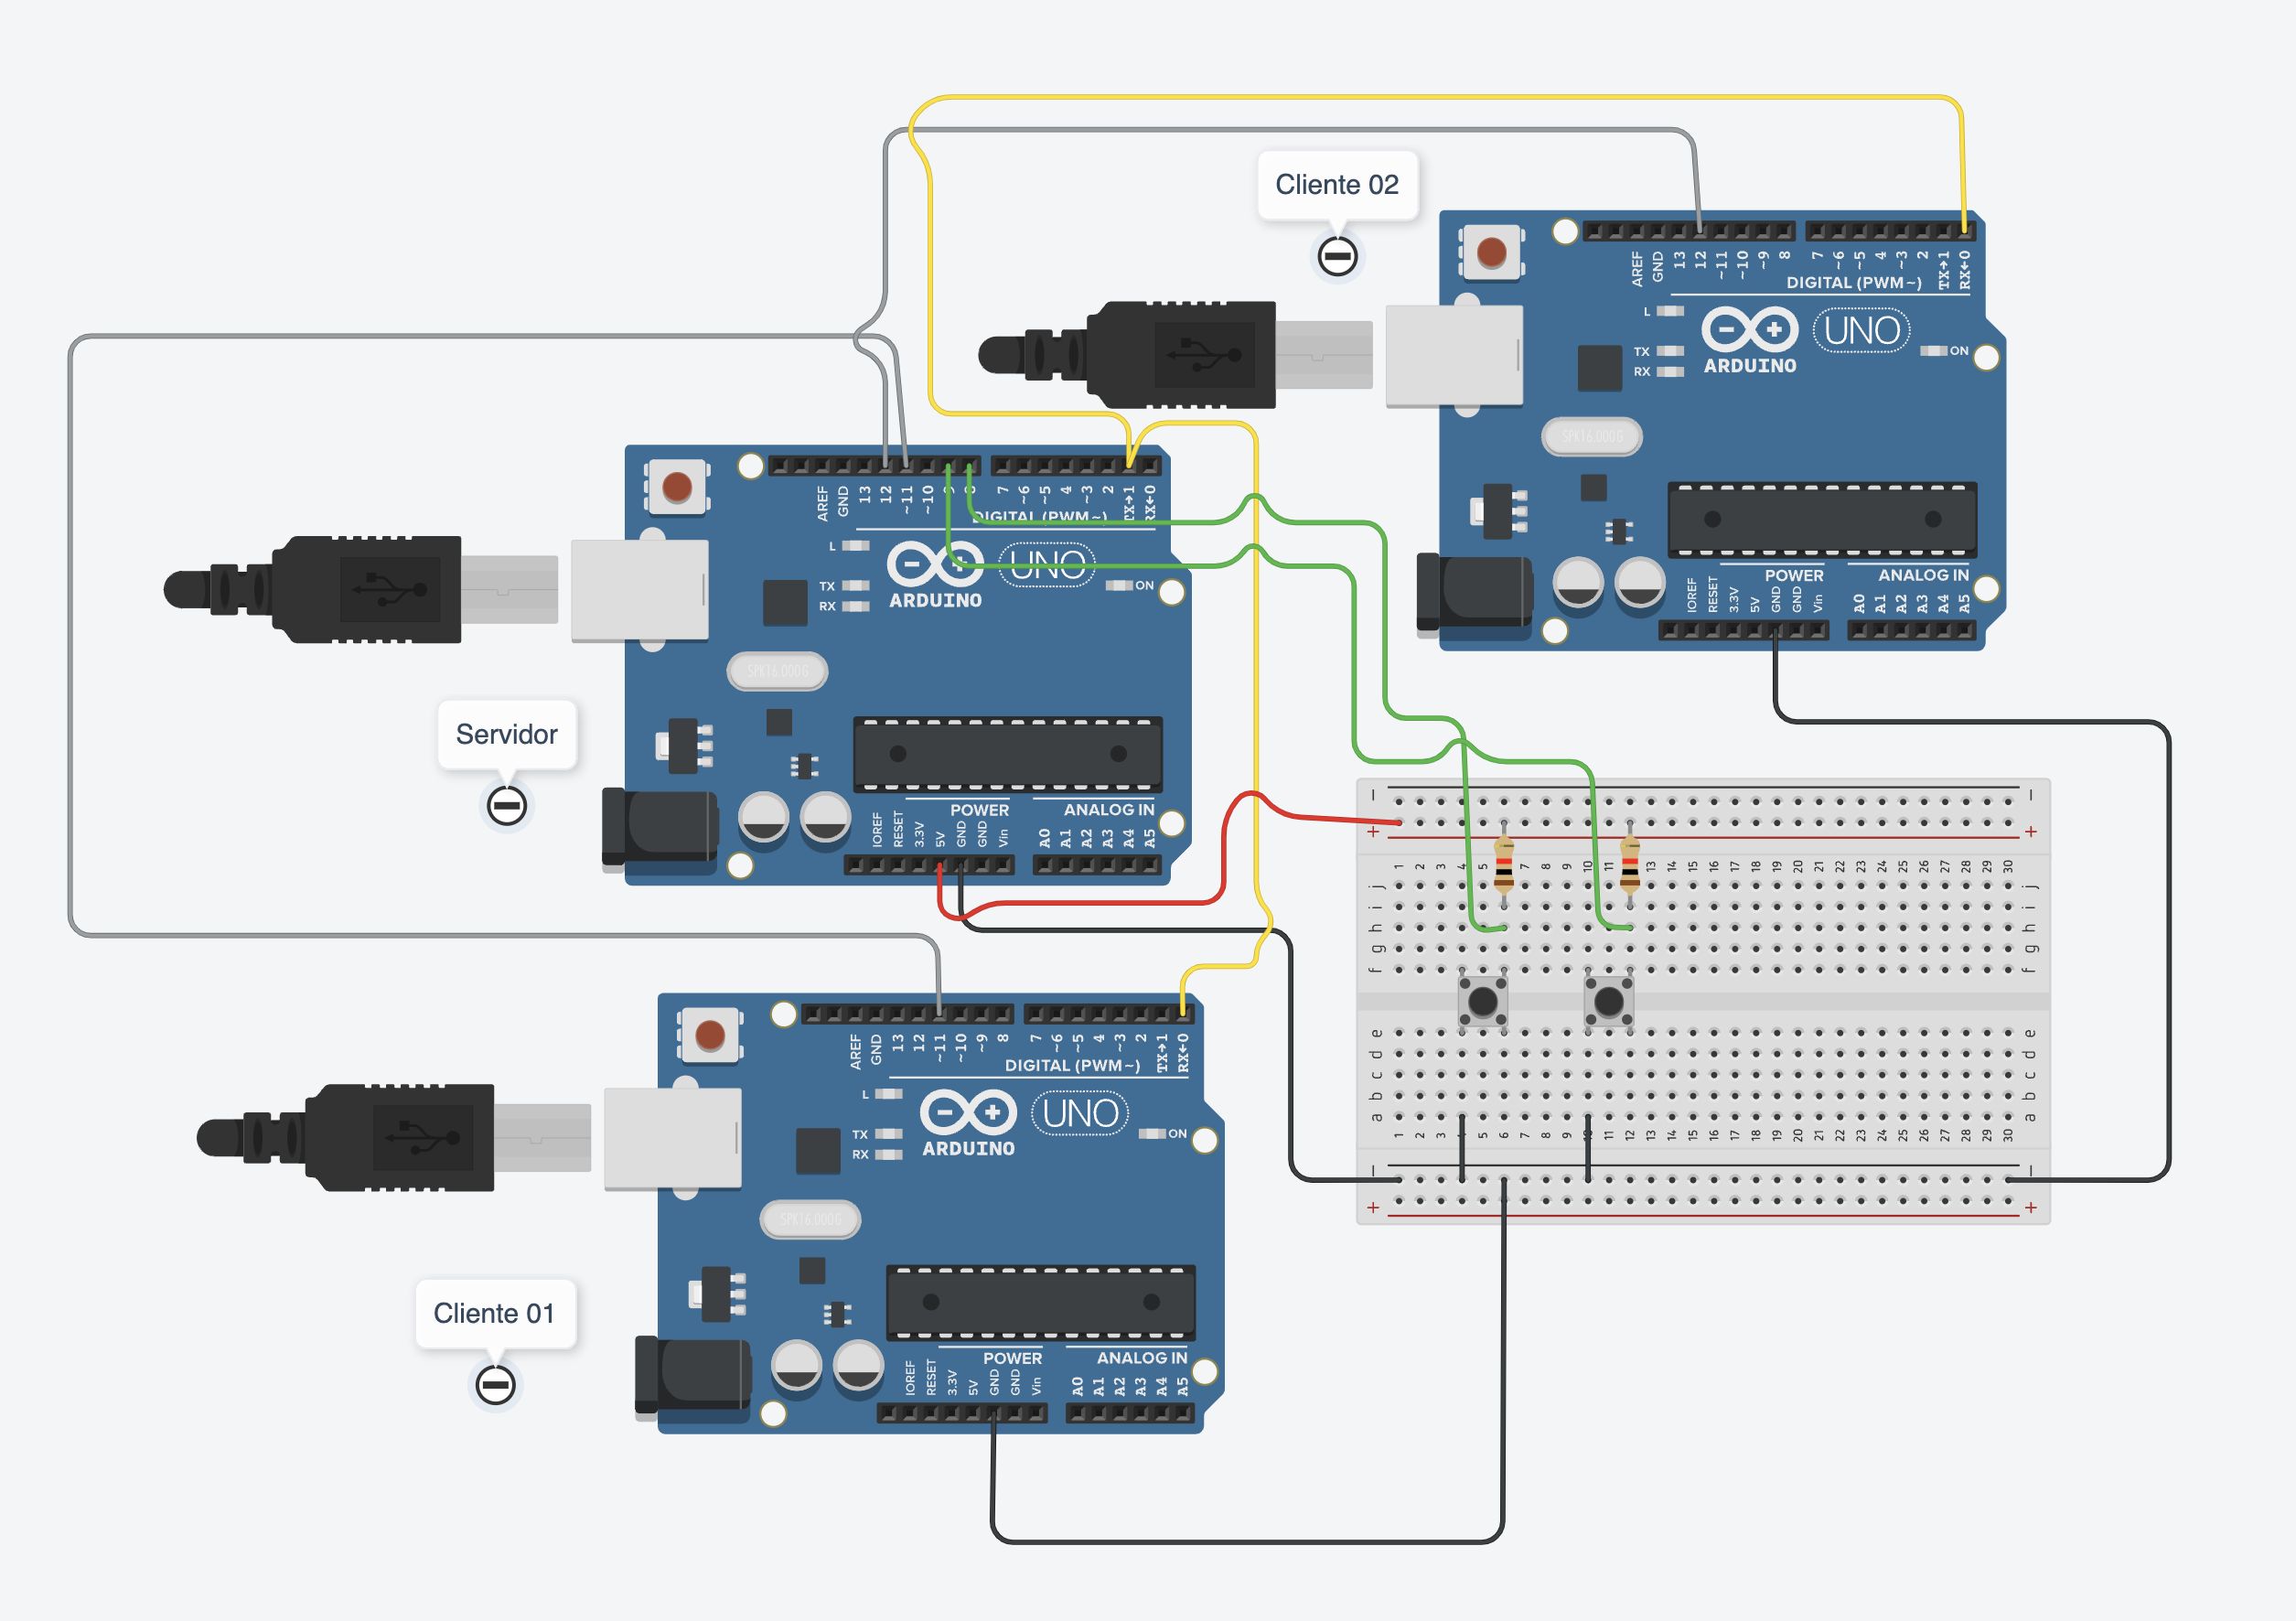
\includegraphics[width=0.8\textwidth]{arduino.png}
	\caption{Montagem final do sistema com os microcontroladores, LEDs e botões no simulador TinkerCAD.}
	\label{fig:resultado}
\end{figure}

\newpage
% -- Conclusion -- %
\begin{center}
	\section{Conclusão}
\end{center}

A implementação de um sistema de comunicação serial entre microcontroladores utilizando a arquitetura Cliente-Servidor demonstrou a eficácia dessa abordagem para o controle e monitoramento de dispositivos em sistemas embarcados. A utilização de GPIOs como Chip Select permitiu a seleção precisa dos dispositivos, garantindo que os comandos fossem direcionados corretamente. A integração de botões físicos para acionar os LEDs mostrou como a interação do usuário pode ser facilmente incorporada em sistemas embarcados. Este trabalho reforça a importância de compreender os conceitos de comunicação serial e arquitetura Cliente-Servidor para o desenvolvimento de soluções eficientes e escaláveis em aplicações de engenharia de controle e automação e engenharia da computação.

\rule{\textwidth}{0.4pt}
\subsubsection{Link do TinkerCAD}
\url{https://www.tinkercad.com/things/5rhsM6DAYVq-brilliant-luulia-elzing/editel?returnTo=https%3A%2F%2Fwww.tinkercad.com%2Fdashboard&sharecode=Q1B5XRHh_h2rFmrkxMFGBgP1fBbbUQ7nosW_mD-sV9Q}


\end{document}
